\documentclass[1p]{elsarticle_modified}
%\bibliographystyle{elsarticle-num}

%\usepackage[colorlinks]{hyperref}
%\usepackage{abbrmath_seonhwa} %\Abb, \Ascr, \Acal ,\Abf, \Afrak
\usepackage{amsfonts}
\usepackage{amssymb}
\usepackage{amsmath}
\usepackage{amsthm}
\usepackage{scalefnt}
\usepackage{amsbsy}
\usepackage{kotex}
\usepackage{caption}
\usepackage{subfig}
\usepackage{color}
\usepackage{graphicx}
\usepackage{xcolor} %% white, black, red, green, blue, cyan, magenta, yellow
\usepackage{float}
\usepackage{setspace}
\usepackage{hyperref}

\usepackage{tikz}
\usetikzlibrary{arrows}

\usepackage{multirow}
\usepackage{array} % fixed length table
\usepackage{hhline}

%%%%%%%%%%%%%%%%%%%%%
\makeatletter
\renewcommand*\env@matrix[1][\arraystretch]{%
	\edef\arraystretch{#1}%
	\hskip -\arraycolsep
	\let\@ifnextchar\new@ifnextchar
	\array{*\c@MaxMatrixCols c}}
\makeatother %https://tex.stackexchange.com/questions/14071/how-can-i-increase-the-line-spacing-in-a-matrix
%%%%%%%%%%%%%%%

\usepackage[normalem]{ulem}

\newcommand{\msout}[1]{\ifmmode\text{\sout{\ensuremath{#1}}}\else\sout{#1}\fi}
%SOURCE: \msout is \stkout macro in https://tex.stackexchange.com/questions/20609/strikeout-in-math-mode

\newcommand{\cancel}[1]{
	\ifmmode
	{\color{red}\msout{#1}}
	\else
	{\color{red}\sout{#1}}
	\fi
}

\newcommand{\add}[1]{
	{\color{blue}\uwave{#1}}
}

\newcommand{\replace}[2]{
	\ifmmode
	{\color{red}\msout{#1}}{\color{blue}\uwave{#2}}
	\else
	{\color{red}\sout{#1}}{\color{blue}\uwave{#2}}
	\fi
}

\newcommand{\Sol}{\mathcal{S}} %segment
\newcommand{\D}{D} %diagram
\newcommand{\A}{\mathcal{A}} %arc


%%%%%%%%%%%%%%%%%%%%%%%%%%%%%5 test

\def\sl{\operatorname{\textup{SL}}(2,\Cbb)}
\def\psl{\operatorname{\textup{PSL}}(2,\Cbb)}
\def\quan{\mkern 1mu \triangleright \mkern 1mu}

\theoremstyle{definition}
\newtheorem{thm}{Theorem}[section]
\newtheorem{prop}[thm]{Proposition}
\newtheorem{lem}[thm]{Lemma}
\newtheorem{ques}[thm]{Question}
\newtheorem{cor}[thm]{Corollary}
\newtheorem{defn}[thm]{Definition}
\newtheorem{exam}[thm]{Example}
\newtheorem{rmk}[thm]{Remark}
\newtheorem{alg}[thm]{Algorithm}

\newcommand{\I}{\sqrt{-1}}
\begin{document}

%\begin{frontmatter}
%
%\title{Boundary parabolic representations of knots up to 8 crossings}
%
%%% Group authors per affiliation:
%\author{Yunhi Cho} 
%\address{Department of Mathematics, University of Seoul, Seoul, Korea}
%\ead{yhcho@uos.ac.kr}
%
%
%\author{Seonhwa Kim} %\fnref{s_kim}}
%\address{Center for Geometry and Physics, Institute for Basic Science, Pohang, 37673, Korea}
%\ead{ryeona17@ibs.re.kr}
%
%\author{Hyuk Kim}
%\address{Department of Mathematical Sciences, Seoul National University, Seoul 08826, Korea}
%\ead{hyukkim@snu.ac.kr}
%
%\author{Seokbeom Yoon}
%\address{Department of Mathematical Sciences, Seoul National University, Seoul, 08826,  Korea}
%\ead{sbyoon15@snu.ac.kr}
%
%\begin{abstract}
%We find all boundary parabolic representation of knots up to 8 crossings.
%
%\end{abstract}
%\begin{keyword}
%    \MSC[2010] 57M25 
%\end{keyword}
%
%\end{frontmatter}

%\linenumbers
%\tableofcontents
%
\newcommand\colored[1]{\textcolor{white}{\rule[-0.35ex]{0.8em}{1.4ex}}\kern-0.8em\color{red} #1}%
%\newcommand\colored[1]{\textcolor{white}{ #1}\kern-2.17ex	\textcolor{white}{ #1}\kern-1.81ex	\textcolor{white}{ #1}\kern-2.15ex\color{red}#1	}

{\Large $\underline{12a_{0423}~(K12a_{0423})}$}

\setlength{\tabcolsep}{10pt}
\renewcommand{\arraystretch}{1.6}
\vspace{1cm}\begin{tabular}{m{100pt}>{\centering\arraybackslash}m{274pt}}
\multirow{5}{120pt}{
	\centering
	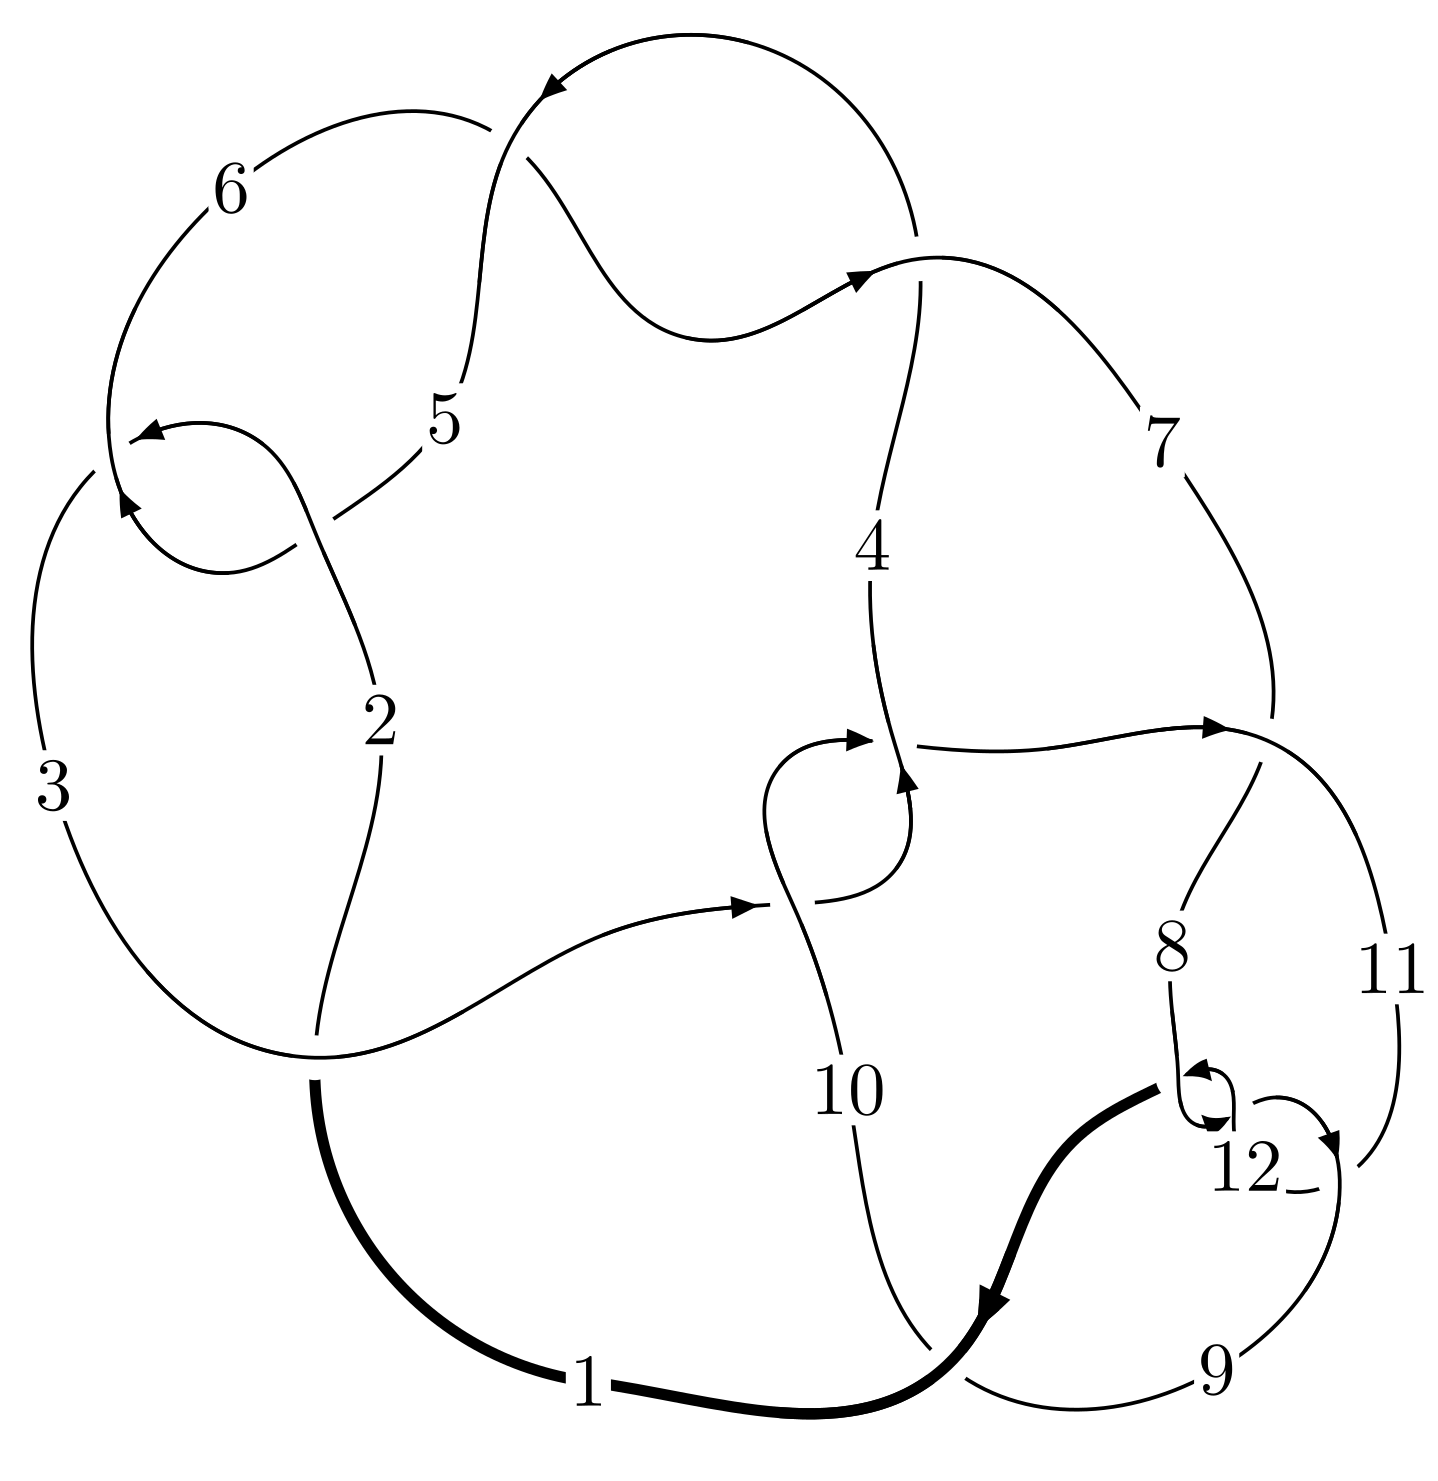
\includegraphics[width=112pt]{../../../GIT/diagram.site/Diagrams/png/1224_12a_0423.png}\\
\ \ \ A knot diagram\footnotemark}&
\allowdisplaybreaks
\textbf{Linearized knot diagam} \\
\cline{2-2}
 &
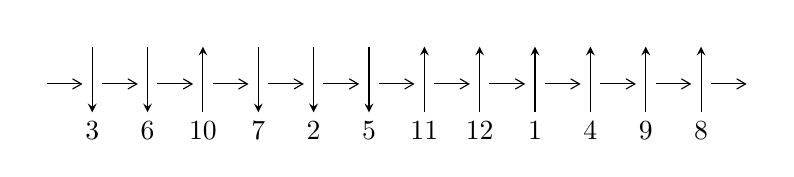
\begin{tikzpicture}[x=20pt, y=17pt]
	% nodes
	\node (C0) at (0, 0) {};
	\node (C1) at (1, 0) {};
	\node (C1U) at (1, +1) {};
	\node (C1D) at (1, -1) {3};

	\node (C2) at (2, 0) {};
	\node (C2U) at (2, +1) {};
	\node (C2D) at (2, -1) {6};

	\node (C3) at (3, 0) {};
	\node (C3U) at (3, +1) {};
	\node (C3D) at (3, -1) {10};

	\node (C4) at (4, 0) {};
	\node (C4U) at (4, +1) {};
	\node (C4D) at (4, -1) {7};

	\node (C5) at (5, 0) {};
	\node (C5U) at (5, +1) {};
	\node (C5D) at (5, -1) {2};

	\node (C6) at (6, 0) {};
	\node (C6U) at (6, +1) {};
	\node (C6D) at (6, -1) {5};

	\node (C7) at (7, 0) {};
	\node (C7U) at (7, +1) {};
	\node (C7D) at (7, -1) {11};

	\node (C8) at (8, 0) {};
	\node (C8U) at (8, +1) {};
	\node (C8D) at (8, -1) {12};

	\node (C9) at (9, 0) {};
	\node (C9U) at (9, +1) {};
	\node (C9D) at (9, -1) {1};

	\node (C10) at (10, 0) {};
	\node (C10U) at (10, +1) {};
	\node (C10D) at (10, -1) {4};

	\node (C11) at (11, 0) {};
	\node (C11U) at (11, +1) {};
	\node (C11D) at (11, -1) {9};

	\node (C12) at (12, 0) {};
	\node (C12U) at (12, +1) {};
	\node (C12D) at (12, -1) {8};
	\node (C13) at (13, 0) {};

	% arrows
	\draw[->,>={angle 60}]
	(C0) edge (C1) (C1) edge (C2) (C2) edge (C3) (C3) edge (C4) (C4) edge (C5) (C5) edge (C6) (C6) edge (C7) (C7) edge (C8) (C8) edge (C9) (C9) edge (C10) (C10) edge (C11) (C11) edge (C12) (C12) edge (C13) ;	\draw[->,>=stealth]
	(C1U) edge (C1D) (C2U) edge (C2D) (C3D) edge (C3U) (C4U) edge (C4D) (C5U) edge (C5D) (C6U) edge (C6D) (C7D) edge (C7U) (C8D) edge (C8U) (C9D) edge (C9U) (C10D) edge (C10U) (C11D) edge (C11U) (C12D) edge (C12U) ;
	\end{tikzpicture} \\
\hhline{~~} \\& 
\textbf{Solving Sequence} \\ \cline{2-2} 
 &
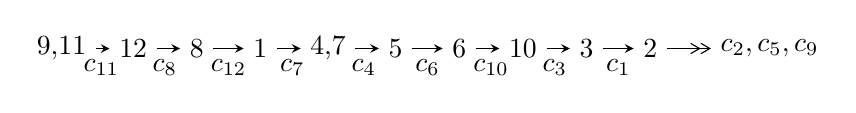
\begin{tikzpicture}[x=23pt, y=7pt]
	% node
	\node (A0) at (-1/8, 0) {9,11};
	\node (A1) at (1, 0) {12};
	\node (A2) at (2, 0) {8};
	\node (A3) at (3, 0) {1};
	\node (A4) at (65/16, 0) {4,7};
	\node (A5) at (41/8, 0) {5};
	\node (A6) at (49/8, 0) {6};
	\node (A7) at (57/8, 0) {10};
	\node (A8) at (65/8, 0) {3};
	\node (A9) at (73/8, 0) {2};
	\node (C1) at (1/2, -1) {$c_{11}$};
	\node (C2) at (3/2, -1) {$c_{8}$};
	\node (C3) at (5/2, -1) {$c_{12}$};
	\node (C4) at (7/2, -1) {$c_{7}$};
	\node (C5) at (37/8, -1) {$c_{4}$};
	\node (C6) at (45/8, -1) {$c_{6}$};
	\node (C7) at (53/8, -1) {$c_{10}$};
	\node (C8) at (61/8, -1) {$c_{3}$};
	\node (C9) at (69/8, -1) {$c_{1}$};
	\node (A10) at (11, 0) {$c_{2},c_{5},c_{9}$};

	% edge
	\draw[->,>=stealth]	
	(A0) edge (A1) (A1) edge (A2) (A2) edge (A3) (A3) edge (A4) (A4) edge (A5) (A5) edge (A6) (A6) edge (A7) (A7) edge (A8) (A8) edge (A9) ;
	\draw[->>,>={angle 60}]	
	(A9) edge (A10);
\end{tikzpicture} \\ 

\end{tabular} \\

\footnotetext{
The image of knot diagram is generated by the software ``\textbf{Draw programme}" developed by Andrew Bartholomew(\url{http://www.layer8.co.uk/maths/draw/index.htm\#Running-draw}), where we modified some parts for our purpose(\url{https://github.com/CATsTAILs/LinksPainter}).
}\phantom \\ \newline 
\centering \textbf{Ideals for irreducible components\footnotemark of $X_{\text{par}}$} 
 
\begin{align*}
I^u_{1}&=\langle 
7 u^{67}+29 u^{66}+\cdots+2 b-5,\;-27 u^{67}-95 u^{66}+\cdots+4 a+37,\;u^{68}+4 u^{67}+\cdots-4 u-1\rangle \\
I^u_{2}&=\langle 
b,\;a^2- a u+2 u^2- u+3,\;u^3- u^2+2 u-1\rangle \\
I^u_{3}&=\langle 
b,\;- u^2+a+u-1,\;u^3- u^2+2 u-1\rangle \\
\\
\end{align*}
\raggedright * 3 irreducible components of $\dim_{\mathbb{C}}=0$, with total 77 representations.\\
\footnotetext{All coefficients of polynomials are rational numbers. But the coefficients are sometimes approximated in decimal forms when there is not enough margin.}
\newpage
\renewcommand{\arraystretch}{1}
\centering \section*{I. $I^u_{1}= \langle 7 u^{67}+29 u^{66}+\cdots+2 b-5,\;-27 u^{67}-95 u^{66}+\cdots+4 a+37,\;u^{68}+4 u^{67}+\cdots-4 u-1 \rangle$}
\flushleft \textbf{(i) Arc colorings}\\
\begin{tabular}{m{7pt} m{180pt} m{7pt} m{180pt} }
\flushright $a_{9}=$&$\begin{pmatrix}0\\u\end{pmatrix}$ \\
\flushright $a_{11}=$&$\begin{pmatrix}1\\0\end{pmatrix}$ \\
\flushright $a_{12}=$&$\begin{pmatrix}1\\- u^2\end{pmatrix}$ \\
\flushright $a_{8}=$&$\begin{pmatrix}- u\\u^3+u\end{pmatrix}$ \\
\flushright $a_{1}=$&$\begin{pmatrix}u^2+1\\- u^4-2 u^2\end{pmatrix}$ \\
\flushright $a_{4}=$&$\begin{pmatrix}\frac{27}{4} u^{67}+\frac{95}{4} u^{66}+\cdots-\frac{51}{2} u-\frac{37}{4}\\-\frac{7}{2} u^{67}-\frac{29}{2} u^{66}+\cdots+11 u+\frac{5}{2}\end{pmatrix}$ \\
\flushright $a_{7}=$&$\begin{pmatrix}- u^3-2 u\\u^3+u\end{pmatrix}$ \\
\flushright $a_{5}=$&$\begin{pmatrix}\frac{9}{2} u^{67}+\frac{31}{2} u^{66}+\cdots-19 u-6\\-\frac{9}{4} u^{67}-10 u^{66}+\cdots+\frac{31}{4} u+\frac{3}{4}\end{pmatrix}$ \\
\flushright $a_{6}=$&$\begin{pmatrix}u^{16}+7 u^{14}+\cdots-6 u+1\\\frac{1}{4} u^{67}+\frac{3}{4} u^{66}+\cdots-\frac{1}{2} u-\frac{1}{4}\end{pmatrix}$ \\
\flushright $a_{10}=$&$\begin{pmatrix}u^5+2 u^3+u\\- u^7-3 u^5-2 u^3+u\end{pmatrix}$ \\
\flushright $a_{3}=$&$\begin{pmatrix}-\frac{3}{4} u^{67}-\frac{3}{4} u^{66}+\cdots-\frac{19}{2} u-\frac{19}{4}\\\frac{5}{2} u^{67}+\frac{21}{2} u^{66}+\cdots-12 u-\frac{9}{2}\end{pmatrix}$ \\
\flushright $a_{2}=$&$\begin{pmatrix}-\frac{1}{4} u^{67}-\frac{3}{4} u^{66}+\cdots+5 u+\frac{1}{2}\\u^{17}+7 u^{15}+\cdots-6 u^2+u\end{pmatrix}$\\&\end{tabular}
\flushleft \textbf{(ii) Obstruction class $= -1$}\\~\\
\flushleft \textbf{(iii) Cusp Shapes $= -\frac{11}{2} u^{67}-\frac{51}{2} u^{66}+\cdots+13 u-\frac{1}{4}$}\\~\\
\newpage\renewcommand{\arraystretch}{1}
\flushleft \textbf{(iv) u-Polynomials at the component}\newline \\
\begin{tabular}{m{50pt}|m{274pt}}
Crossings & \hspace{64pt}u-Polynomials at each crossing \\
\hline $$\begin{aligned}c_{1},c_{4},c_{6}\end{aligned}$$&$\begin{aligned}
&u^{68}+16 u^{67}+\cdots+28 u+1
\end{aligned}$\\
\hline $$\begin{aligned}c_{2},c_{5}\end{aligned}$$&$\begin{aligned}
&u^{68}+4 u^{67}+\cdots+4 u-1
\end{aligned}$\\
\hline $$\begin{aligned}c_{3},c_{10}\end{aligned}$$&$\begin{aligned}
&u^{68}+u^{67}+\cdots+1536 u+512
\end{aligned}$\\
\hline $$\begin{aligned}c_{7},c_{9}\end{aligned}$$&$\begin{aligned}
&u^{68}-4 u^{67}+\cdots+298 u-193
\end{aligned}$\\
\hline $$\begin{aligned}c_{8},c_{11},c_{12}\end{aligned}$$&$\begin{aligned}
&u^{68}+4 u^{67}+\cdots-4 u-1
\end{aligned}$\\
\hline
\end{tabular}\\~\\
\newpage\renewcommand{\arraystretch}{1}
\flushleft \textbf{(v) Riley Polynomials at the component}\newline \\
\begin{tabular}{m{50pt}|m{274pt}}
Crossings & \hspace{64pt}Riley Polynomials at each crossing \\
\hline $$\begin{aligned}c_{1},c_{4},c_{6}\end{aligned}$$&$\begin{aligned}
&y^{68}+76 y^{67}+\cdots-468 y+1
\end{aligned}$\\
\hline $$\begin{aligned}c_{2},c_{5}\end{aligned}$$&$\begin{aligned}
&y^{68}-16 y^{67}+\cdots-28 y+1
\end{aligned}$\\
\hline $$\begin{aligned}c_{3},c_{10}\end{aligned}$$&$\begin{aligned}
&y^{68}-49 y^{67}+\cdots-3276800 y+262144
\end{aligned}$\\
\hline $$\begin{aligned}c_{7},c_{9}\end{aligned}$$&$\begin{aligned}
&y^{68}-56 y^{67}+\cdots+843772 y+37249
\end{aligned}$\\
\hline $$\begin{aligned}c_{8},c_{11},c_{12}\end{aligned}$$&$\begin{aligned}
&y^{68}+56 y^{67}+\cdots+12 y+1
\end{aligned}$\\
\hline
\end{tabular}\\~\\
\newpage\flushleft \textbf{(vi) Complex Volumes and Cusp Shapes}
$$\begin{array}{c|c|c}  
\text{Solutions to }I^u_{1}& \I (\text{vol} + \sqrt{-1}CS) & \text{Cusp shape}\\
 \hline 
\begin{aligned}
u &= -0.883196 + 0.110879 I \\
a &= \phantom{-}2.28702 + 0.20938 I \\
b &= -1.54451 + 0.55845 I\end{aligned}
 & \phantom{-}14.5227 - 3.6785 I & \phantom{-}9.66151 + 1.29736 I \\ \hline\begin{aligned}
u &= -0.883196 - 0.110879 I \\
a &= \phantom{-}2.28702 - 0.20938 I \\
b &= -1.54451 - 0.55845 I\end{aligned}
 & \phantom{-}14.5227 + 3.6785 I & \phantom{-}9.66151 - 1.29736 I \\ \hline\begin{aligned}
u &= -0.878083 + 0.122555 I \\
a &= -2.27299 - 0.23480 I \\
b &= \phantom{-}1.50934 - 0.61168 I\end{aligned}
 & \phantom{-}14.0779 - 10.2341 I & \phantom{-}8.93592 + 6.05514 I \\ \hline\begin{aligned}
u &= -0.878083 - 0.122555 I \\
a &= -2.27299 + 0.23480 I \\
b &= \phantom{-}1.50934 + 0.61168 I\end{aligned}
 & \phantom{-}14.0779 + 10.2341 I & \phantom{-}8.93592 - 6.05514 I \\ \hline\begin{aligned}
u &= -0.842036 + 0.041084 I \\
a &= \phantom{-}2.47425 + 0.12172 I \\
b &= -1.380970 + 0.196665 I\end{aligned}
 & \phantom{-}7.31201 - 1.61336 I & \phantom{-}10.65283 + 0.71053 I \\ \hline\begin{aligned}
u &= -0.842036 - 0.041084 I \\
a &= \phantom{-}2.47425 - 0.12172 I \\
b &= -1.380970 - 0.196665 I\end{aligned}
 & \phantom{-}7.31201 + 1.61336 I & \phantom{-}10.65283 - 0.71053 I \\ \hline\begin{aligned}
u &= \phantom{-}0.836342 + 0.008912 I \\
a &= -0.017629 + 1.041540 I \\
b &= \phantom{-}0.042391 - 1.358950 I\end{aligned}
 & \phantom{-}9.34458 + 3.20678 I & \phantom{-}8.45402 - 2.50897 I \\ \hline\begin{aligned}
u &= \phantom{-}0.836342 - 0.008912 I \\
a &= -0.017629 - 1.041540 I \\
b &= \phantom{-}0.042391 + 1.358950 I\end{aligned}
 & \phantom{-}9.34458 - 3.20678 I & \phantom{-}8.45402 + 2.50897 I \\ \hline\begin{aligned}
u &= -0.820055 + 0.078945 I \\
a &= -2.47808 - 0.26474 I \\
b &= \phantom{-}1.263950 - 0.365738 I\end{aligned}
 & \phantom{-}5.17218 - 6.11204 I & \phantom{-}6.64053 + 6.47258 I \\ \hline\begin{aligned}
u &= -0.820055 - 0.078945 I \\
a &= -2.47808 + 0.26474 I \\
b &= \phantom{-}1.263950 + 0.365738 I\end{aligned}
 & \phantom{-}5.17218 + 6.11204 I & \phantom{-}6.64053 - 6.47258 I\\
 \hline 
 \end{array}$$\newpage$$\begin{array}{c|c|c}  
\text{Solutions to }I^u_{1}& \I (\text{vol} + \sqrt{-1}CS) & \text{Cusp shape}\\
 \hline 
\begin{aligned}
u &= -0.074714 + 1.188830 I \\
a &= \phantom{-}0.891353 - 1.049750 I \\
b &= -0.638314 - 0.584251 I\end{aligned}
 & \phantom{-}0.28440 + 1.43816 I & \phantom{-0.000000 } 0 \\ \hline\begin{aligned}
u &= -0.074714 - 1.188830 I \\
a &= \phantom{-}0.891353 + 1.049750 I \\
b &= -0.638314 + 0.584251 I\end{aligned}
 & \phantom{-}0.28440 - 1.43816 I & \phantom{-0.000000 } 0 \\ \hline\begin{aligned}
u &= -0.789953\phantom{ +0.000000I} \\
a &= -2.69327\phantom{ +0.000000I} \\
b &= \phantom{-}1.14488\phantom{ +0.000000I}\end{aligned}
 & \phantom{-}2.31303\phantom{ +0.000000I} & \phantom{-}4.51890\phantom{ +0.000000I} \\ \hline\begin{aligned}
u &= \phantom{-}0.576977 + 0.530503 I \\
a &= \phantom{-}0.824531 - 0.923493 I \\
b &= -1.359680 - 0.151800 I\end{aligned}
 & \phantom{-}8.22238 + 5.29147 I & \phantom{-}7.35195 - 5.78163 I \\ \hline\begin{aligned}
u &= \phantom{-}0.576977 - 0.530503 I \\
a &= \phantom{-}0.824531 + 0.923493 I \\
b &= -1.359680 + 0.151800 I\end{aligned}
 & \phantom{-}8.22238 - 5.29147 I & \phantom{-}7.35195 + 5.78163 I \\ \hline\begin{aligned}
u &= \phantom{-}0.593054 + 0.504319 I \\
a &= -0.807717 + 0.928418 I \\
b &= \phantom{-}1.357810 + 0.068287 I\end{aligned}
 & \phantom{-}8.30625 - 1.12217 I & \phantom{-}7.67861 - 0.76629 I \\ \hline\begin{aligned}
u &= \phantom{-}0.593054 - 0.504319 I \\
a &= -0.807717 - 0.928418 I \\
b &= \phantom{-}1.357810 - 0.068287 I\end{aligned}
 & \phantom{-}8.30625 + 1.12217 I & \phantom{-}7.67861 + 0.76629 I \\ \hline\begin{aligned}
u &= -0.448687 + 1.144800 I \\
a &= \phantom{-}0.709101 + 0.607422 I \\
b &= -1.54402 - 0.50394 I\end{aligned}
 & \phantom{-}10.94400 + 5.49512 I & \phantom{-0.000000 } 0 \\ \hline\begin{aligned}
u &= -0.448687 - 1.144800 I \\
a &= \phantom{-}0.709101 - 0.607422 I \\
b &= -1.54402 + 0.50394 I\end{aligned}
 & \phantom{-}10.94400 - 5.49512 I & \phantom{-0.000000 } 0 \\ \hline\begin{aligned}
u &= -0.081643 + 1.234740 I \\
a &= -0.87255 + 1.30038 I \\
b &= \phantom{-}0.594137 + 0.582932 I\end{aligned}
 & -0.15037 - 4.30964 I & \phantom{-0.000000 } 0\\
 \hline 
 \end{array}$$\newpage$$\begin{array}{c|c|c}  
\text{Solutions to }I^u_{1}& \I (\text{vol} + \sqrt{-1}CS) & \text{Cusp shape}\\
 \hline 
\begin{aligned}
u &= -0.081643 - 1.234740 I \\
a &= -0.87255 - 1.30038 I \\
b &= \phantom{-}0.594137 - 0.582932 I\end{aligned}
 & -0.15037 + 4.30964 I & \phantom{-0.000000 } 0 \\ \hline\begin{aligned}
u &= -0.357510 + 1.191950 I \\
a &= \phantom{-}1.211980 + 0.542043 I \\
b &= -1.229020 - 0.227598 I\end{aligned}
 & \phantom{-}1.76607 + 1.85694 I & \phantom{-0.000000 } 0 \\ \hline\begin{aligned}
u &= -0.357510 - 1.191950 I \\
a &= \phantom{-}1.211980 - 0.542043 I \\
b &= -1.229020 + 0.227598 I\end{aligned}
 & \phantom{-}1.76607 - 1.85694 I & \phantom{-0.000000 } 0 \\ \hline\begin{aligned}
u &= -0.449847 + 1.160780 I \\
a &= -0.740080 - 0.666202 I \\
b &= \phantom{-}1.57548 + 0.44356 I\end{aligned}
 & \phantom{-}11.30140 - 1.07993 I & \phantom{-0.000000 } 0 \\ \hline\begin{aligned}
u &= -0.449847 - 1.160780 I \\
a &= -0.740080 + 0.666202 I \\
b &= \phantom{-}1.57548 - 0.44356 I\end{aligned}
 & \phantom{-}11.30140 + 1.07993 I & \phantom{-0.000000 } 0 \\ \hline\begin{aligned}
u &= \phantom{-}0.273567 + 1.231890 I \\
a &= \phantom{-}0.610435 - 0.305888 I \\
b &= -0.123364 - 0.850513 I\end{aligned}
 & -1.79566 + 1.87689 I & \phantom{-0.000000 } 0 \\ \hline\begin{aligned}
u &= \phantom{-}0.273567 - 1.231890 I \\
a &= \phantom{-}0.610435 + 0.305888 I \\
b &= -0.123364 + 0.850513 I\end{aligned}
 & -1.79566 - 1.87689 I & \phantom{-0.000000 } 0 \\ \hline\begin{aligned}
u &= \phantom{-}0.114749 + 1.267340 I \\
a &= \phantom{-}0.241747 - 0.755643 I \\
b &= -0.563150 - 0.524155 I\end{aligned}
 & -3.19195 + 1.95948 I & \phantom{-0.000000 } 0 \\ \hline\begin{aligned}
u &= \phantom{-}0.114749 - 1.267340 I \\
a &= \phantom{-}0.241747 + 0.755643 I \\
b &= -0.563150 + 0.524155 I\end{aligned}
 & -3.19195 - 1.95948 I & \phantom{-0.000000 } 0 \\ \hline\begin{aligned}
u &= \phantom{-}0.718407 + 0.054666 I \\
a &= -0.136876 + 0.792692 I \\
b &= \phantom{-}0.229382 - 0.831076 I\end{aligned}
 & \phantom{-}1.79469 + 1.70423 I & \phantom{-}5.68933 - 4.03428 I\\
 \hline 
 \end{array}$$\newpage$$\begin{array}{c|c|c}  
\text{Solutions to }I^u_{1}& \I (\text{vol} + \sqrt{-1}CS) & \text{Cusp shape}\\
 \hline 
\begin{aligned}
u &= \phantom{-}0.718407 - 0.054666 I \\
a &= -0.136876 - 0.792692 I \\
b &= \phantom{-}0.229382 + 0.831076 I\end{aligned}
 & \phantom{-}1.79469 - 1.70423 I & \phantom{-}5.68933 + 4.03428 I \\ \hline\begin{aligned}
u &= -0.386268 + 1.231950 I \\
a &= -1.17649 - 0.83959 I \\
b &= \phantom{-}1.372460 + 0.057138 I\end{aligned}
 & \phantom{-}3.63723 - 2.79864 I & \phantom{-0.000000 } 0 \\ \hline\begin{aligned}
u &= -0.386268 - 1.231950 I \\
a &= -1.17649 + 0.83959 I \\
b &= \phantom{-}1.372460 - 0.057138 I\end{aligned}
 & \phantom{-}3.63723 + 2.79864 I & \phantom{-0.000000 } 0 \\ \hline\begin{aligned}
u &= \phantom{-}0.015638 + 1.299180 I \\
a &= -0.263537 + 1.187850 I \\
b &= \phantom{-}0.654251 + 0.629382 I\end{aligned}
 & -5.82782 - 0.26682 I & \phantom{-0.000000 } 0 \\ \hline\begin{aligned}
u &= \phantom{-}0.015638 - 1.299180 I \\
a &= -0.263537 - 1.187850 I \\
b &= \phantom{-}0.654251 - 0.629382 I\end{aligned}
 & -5.82782 + 0.26682 I & \phantom{-0.000000 } 0 \\ \hline\begin{aligned}
u &= \phantom{-}0.380086 + 1.262700 I \\
a &= \phantom{-}0.897471 - 0.203783 I \\
b &= \phantom{-}0.103923 - 1.353660 I\end{aligned}
 & \phantom{-}5.45713 + 1.16252 I & \phantom{-0.000000 } 0 \\ \hline\begin{aligned}
u &= \phantom{-}0.380086 - 1.262700 I \\
a &= \phantom{-}0.897471 + 0.203783 I \\
b &= \phantom{-}0.103923 + 1.353660 I\end{aligned}
 & \phantom{-}5.45713 - 1.16252 I & \phantom{-0.000000 } 0 \\ \hline\begin{aligned}
u &= -0.344177 + 1.273700 I \\
a &= \phantom{-}1.53531 + 1.04902 I \\
b &= -1.156260 + 0.164863 I\end{aligned}
 & -1.64536 - 4.08494 I & \phantom{-0.000000 } 0 \\ \hline\begin{aligned}
u &= -0.344177 - 1.273700 I \\
a &= \phantom{-}1.53531 - 1.04902 I \\
b &= -1.156260 - 0.164863 I\end{aligned}
 & -1.64536 + 4.08494 I & \phantom{-0.000000 } 0 \\ \hline\begin{aligned}
u &= \phantom{-}0.378704 + 1.277060 I \\
a &= -0.901537 + 0.167233 I \\
b &= -0.183952 + 1.350690 I\end{aligned}
 & \phantom{-}5.34738 + 7.57130 I & \phantom{-0.000000 } 0\\
 \hline 
 \end{array}$$\newpage$$\begin{array}{c|c|c}  
\text{Solutions to }I^u_{1}& \I (\text{vol} + \sqrt{-1}CS) & \text{Cusp shape}\\
 \hline 
\begin{aligned}
u &= \phantom{-}0.378704 - 1.277060 I \\
a &= -0.901537 - 0.167233 I \\
b &= -0.183952 - 1.350690 I\end{aligned}
 & \phantom{-}5.34738 - 7.57130 I & \phantom{-0.000000 } 0 \\ \hline\begin{aligned}
u &= \phantom{-}0.299464 + 1.300730 I \\
a &= -0.671330 + 0.054559 I \\
b &= -0.290086 + 0.868205 I\end{aligned}
 & -2.44438 + 5.38952 I & \phantom{-0.000000 } 0 \\ \hline\begin{aligned}
u &= \phantom{-}0.299464 - 1.300730 I \\
a &= -0.671330 - 0.054559 I \\
b &= -0.290086 - 0.868205 I\end{aligned}
 & -2.44438 - 5.38952 I & \phantom{-0.000000 } 0 \\ \hline\begin{aligned}
u &= -0.380669 + 1.300130 I \\
a &= -1.27591 - 1.24442 I \\
b &= \phantom{-}1.369760 - 0.318562 I\end{aligned}
 & \phantom{-}3.12774 - 6.00570 I & \phantom{-0.000000 } 0 \\ \hline\begin{aligned}
u &= -0.380669 - 1.300130 I \\
a &= -1.27591 + 1.24442 I \\
b &= \phantom{-}1.369760 + 0.318562 I\end{aligned}
 & \phantom{-}3.12774 + 6.00570 I & \phantom{-0.000000 } 0 \\ \hline\begin{aligned}
u &= \phantom{-}0.217986 + 1.345040 I \\
a &= -0.350229 - 0.323689 I \\
b &= -0.564549 + 0.170572 I\end{aligned}
 & -3.80220 + 2.41064 I & \phantom{-0.000000 } 0 \\ \hline\begin{aligned}
u &= \phantom{-}0.217986 - 1.345040 I \\
a &= -0.350229 + 0.323689 I \\
b &= -0.564549 - 0.170572 I\end{aligned}
 & -3.80220 - 2.41064 I & \phantom{-0.000000 } 0 \\ \hline\begin{aligned}
u &= \phantom{-}0.093295 + 1.367930 I \\
a &= \phantom{-}0.160591 + 0.969459 I \\
b &= \phantom{-}0.835398 + 0.483273 I\end{aligned}
 & -5.23627 + 4.58427 I & \phantom{-0.000000 } 0 \\ \hline\begin{aligned}
u &= \phantom{-}0.093295 - 1.367930 I \\
a &= \phantom{-}0.160591 - 0.969459 I \\
b &= \phantom{-}0.835398 - 0.483273 I\end{aligned}
 & -5.23627 - 4.58427 I & \phantom{-0.000000 } 0 \\ \hline\begin{aligned}
u &= -0.364104 + 1.323200 I \\
a &= \phantom{-}1.35385 + 1.40669 I \\
b &= -1.271370 + 0.466726 I\end{aligned}
 & \phantom{-}0.77875 - 10.37800 I & \phantom{-0.000000 } 0\\
 \hline 
 \end{array}$$\newpage$$\begin{array}{c|c|c}  
\text{Solutions to }I^u_{1}& \I (\text{vol} + \sqrt{-1}CS) & \text{Cusp shape}\\
 \hline 
\begin{aligned}
u &= -0.364104 - 1.323200 I \\
a &= \phantom{-}1.35385 - 1.40669 I \\
b &= -1.271370 - 0.466726 I\end{aligned}
 & \phantom{-}0.77875 + 10.37800 I & \phantom{-0.000000 } 0 \\ \hline\begin{aligned}
u &= -0.395915 + 1.350660 I \\
a &= -1.13840 - 1.49595 I \\
b &= \phantom{-}1.49290 - 0.63680 I\end{aligned}
 & \phantom{-}9.93330 - 8.26771 I & \phantom{-0.000000 } 0 \\ \hline\begin{aligned}
u &= -0.395915 - 1.350660 I \\
a &= -1.13840 + 1.49595 I \\
b &= \phantom{-}1.49290 + 0.63680 I\end{aligned}
 & \phantom{-}9.93330 + 8.26771 I & \phantom{-0.000000 } 0 \\ \hline\begin{aligned}
u &= -0.390304 + 1.356620 I \\
a &= \phantom{-}1.15307 + 1.53169 I \\
b &= -1.45794 + 0.68098 I\end{aligned}
 & \phantom{-}9.4275 - 14.7877 I & \phantom{-0.000000 } 0 \\ \hline\begin{aligned}
u &= -0.390304 - 1.356620 I \\
a &= \phantom{-}1.15307 - 1.53169 I \\
b &= -1.45794 - 0.68098 I\end{aligned}
 & \phantom{-}9.4275 + 14.7877 I & \phantom{-0.000000 } 0 \\ \hline\begin{aligned}
u &= \phantom{-}0.341611 + 0.461012 I \\
a &= \phantom{-}0.861805 - 0.885756 I \\
b &= -0.878881 - 0.293282 I\end{aligned}
 & \phantom{-}0.40677 + 3.17475 I & \phantom{-}3.07710 - 8.65765 I \\ \hline\begin{aligned}
u &= \phantom{-}0.341611 - 0.461012 I \\
a &= \phantom{-}0.861805 + 0.885756 I \\
b &= -0.878881 + 0.293282 I\end{aligned}
 & \phantom{-}0.40677 - 3.17475 I & \phantom{-}3.07710 + 8.65765 I \\ \hline\begin{aligned}
u &= \phantom{-}0.498530 + 0.267549 I \\
a &= -0.756073 + 0.717769 I \\
b &= \phantom{-}0.795737 - 0.123613 I\end{aligned}
 & \phantom{-}1.109940 - 0.236478 I & \phantom{-}7.83765 + 0.33377 I \\ \hline\begin{aligned}
u &= \phantom{-}0.498530 - 0.267549 I \\
a &= -0.756073 - 0.717769 I \\
b &= \phantom{-}0.795737 + 0.123613 I\end{aligned}
 & \phantom{-}1.109940 + 0.236478 I & \phantom{-}7.83765 - 0.33377 I \\ \hline\begin{aligned}
u &= \phantom{-}0.15691 + 1.43163 I \\
a &= -0.531513 - 0.823143 I \\
b &= -1.167860 - 0.205420 I\end{aligned}
 & \phantom{-}2.05830 + 1.37245 I & \phantom{-0.000000 } 0\\
 \hline 
 \end{array}$$\newpage$$\begin{array}{c|c|c}  
\text{Solutions to }I^u_{1}& \I (\text{vol} + \sqrt{-1}CS) & \text{Cusp shape}\\
 \hline 
\begin{aligned}
u &= \phantom{-}0.15691 - 1.43163 I \\
a &= -0.531513 + 0.823143 I \\
b &= -1.167860 + 0.205420 I\end{aligned}
 & \phantom{-}2.05830 - 1.37245 I & \phantom{-0.000000 } 0 \\ \hline\begin{aligned}
u &= \phantom{-}0.14259 + 1.43508 I \\
a &= \phantom{-}0.516840 + 0.882774 I \\
b &= \phantom{-}1.175310 + 0.290911 I\end{aligned}
 & \phantom{-}1.86781 + 7.64221 I & \phantom{-0.000000 } 0 \\ \hline\begin{aligned}
u &= \phantom{-}0.14259 - 1.43508 I \\
a &= \phantom{-}0.516840 - 0.882774 I \\
b &= \phantom{-}1.175310 - 0.290911 I\end{aligned}
 & \phantom{-}1.86781 - 7.64221 I & \phantom{-0.000000 } 0 \\ \hline\begin{aligned}
u &= \phantom{-}0.459924\phantom{ +0.000000I} \\
a &= -0.727898\phantom{ +0.000000I} \\
b &= \phantom{-}0.446382\phantom{ +0.000000I}\end{aligned}
 & \phantom{-}0.791286\phantom{ +0.000000I} & \phantom{-}12.9510\phantom{ +0.000000I} \\ \hline\begin{aligned}
u &= -0.327604 + 0.031735 I \\
a &= -0.07580 - 2.80687 I \\
b &= -0.005736 - 0.498706 I\end{aligned}
 & \phantom{-}3.56841 - 2.90168 I & -2.97092 + 3.54606 I \\ \hline\begin{aligned}
u &= -0.327604 - 0.031735 I \\
a &= -0.07580 + 2.80687 I \\
b &= -0.005736 + 0.498706 I\end{aligned}
 & \phantom{-}3.56841 + 2.90168 I & -2.97092 - 3.54606 I \\ \hline\begin{aligned}
u &= -0.048081 + 0.224645 I \\
a &= \phantom{-}0.94797 - 1.88047 I \\
b &= -0.308184 - 0.394663 I\end{aligned}
 & -1.259210 - 0.317933 I & -6.24438 + 0.78722 I \\ \hline\begin{aligned}
u &= -0.048081 - 0.224645 I \\
a &= \phantom{-}0.94797 + 1.88047 I \\
b &= -0.308184 + 0.394663 I\end{aligned}
 & -1.259210 + 0.317933 I & -6.24438 - 0.78722 I\\
 \hline 
 \end{array}$$\newpage\newpage\renewcommand{\arraystretch}{1}
\centering \section*{II. $I^u_{2}= \langle b,\;a^2- a u+2 u^2- u+3,\;u^3- u^2+2 u-1 \rangle$}
\flushleft \textbf{(i) Arc colorings}\\
\begin{tabular}{m{7pt} m{180pt} m{7pt} m{180pt} }
\flushright $a_{9}=$&$\begin{pmatrix}0\\u\end{pmatrix}$ \\
\flushright $a_{11}=$&$\begin{pmatrix}1\\0\end{pmatrix}$ \\
\flushright $a_{12}=$&$\begin{pmatrix}1\\- u^2\end{pmatrix}$ \\
\flushright $a_{8}=$&$\begin{pmatrix}- u\\u^2- u+1\end{pmatrix}$ \\
\flushright $a_{1}=$&$\begin{pmatrix}u^2+1\\- u^2+u-1\end{pmatrix}$ \\
\flushright $a_{4}=$&$\begin{pmatrix}a\\0\end{pmatrix}$ \\
\flushright $a_{7}=$&$\begin{pmatrix}- u^2-1\\u^2- u+1\end{pmatrix}$ \\
\flushright $a_{5}=$&$\begin{pmatrix}0\\a u\end{pmatrix}$ \\
\flushright $a_{6}=$&$\begin{pmatrix}- u^2-1\\- u^2 a+a u- u\end{pmatrix}$ \\
\flushright $a_{10}=$&$\begin{pmatrix}1\\0\end{pmatrix}$ \\
\flushright $a_{3}=$&$\begin{pmatrix}a\\0\end{pmatrix}$ \\
\flushright $a_{2}=$&$\begin{pmatrix}- a u+a-1\\- u^2+u-1\end{pmatrix}$\\&\end{tabular}
\flushleft \textbf{(ii) Obstruction class $= 1$}\\~\\
\flushleft \textbf{(iii) Cusp Shapes $= -2 u^2 a-2 a u+10 u^2+3 a-12 u+15$}\\~\\
\newpage\renewcommand{\arraystretch}{1}
\flushleft \textbf{(iv) u-Polynomials at the component}\newline \\
\begin{tabular}{m{50pt}|m{274pt}}
Crossings & \hspace{64pt}u-Polynomials at each crossing \\
\hline $$\begin{aligned}c_{1},c_{4},c_{11}\\c_{12}\end{aligned}$$&$\begin{aligned}
&(u^3- u^2+2 u-1)^2
\end{aligned}$\\
\hline $$\begin{aligned}c_{2}\end{aligned}$$&$\begin{aligned}
&(u^3+u^2-1)^2
\end{aligned}$\\
\hline $$\begin{aligned}c_{3},c_{10}\end{aligned}$$&$\begin{aligned}
&u^6
\end{aligned}$\\
\hline $$\begin{aligned}c_{5},c_{7},c_{9}\end{aligned}$$&$\begin{aligned}
&(u^3- u^2+1)^2
\end{aligned}$\\
\hline $$\begin{aligned}c_{6},c_{8}\end{aligned}$$&$\begin{aligned}
&(u^3+u^2+2 u+1)^2
\end{aligned}$\\
\hline
\end{tabular}\\~\\
\newpage\renewcommand{\arraystretch}{1}
\flushleft \textbf{(v) Riley Polynomials at the component}\newline \\
\begin{tabular}{m{50pt}|m{274pt}}
Crossings & \hspace{64pt}Riley Polynomials at each crossing \\
\hline $$\begin{aligned}c_{1},c_{4},c_{6}\\c_{8},c_{11},c_{12}\end{aligned}$$&$\begin{aligned}
&(y^3+3 y^2+2 y-1)^2
\end{aligned}$\\
\hline $$\begin{aligned}c_{2},c_{5},c_{7}\\c_{9}\end{aligned}$$&$\begin{aligned}
&(y^3- y^2+2 y-1)^2
\end{aligned}$\\
\hline $$\begin{aligned}c_{3},c_{10}\end{aligned}$$&$\begin{aligned}
&y^6
\end{aligned}$\\
\hline
\end{tabular}\\~\\
\newpage\flushleft \textbf{(vi) Complex Volumes and Cusp Shapes}
$$\begin{array}{c|c|c}  
\text{Solutions to }I^u_{2}& \I (\text{vol} + \sqrt{-1}CS) & \text{Cusp shape}\\
 \hline 
\begin{aligned}
u &= \phantom{-}0.215080 + 1.307140 I \\
a &= \phantom{-}0.592519 + 0.986732 I \\
b &= \phantom{-0.000000 } 0\end{aligned}
 & \phantom{-0.000000 -}5.65624 I & \phantom{-}2.97732 - 6.46189 I \\ \hline\begin{aligned}
u &= \phantom{-}0.215080 + 1.307140 I \\
a &= -0.377439 + 0.320410 I \\
b &= \phantom{-0.000000 } 0\end{aligned}
 & -4.13758 + 2.82812 I & -5.23142 - 6.76304 I \\ \hline\begin{aligned}
u &= \phantom{-}0.215080 - 1.307140 I \\
a &= \phantom{-}0.592519 - 0.986732 I \\
b &= \phantom{-0.000000 } 0\end{aligned}
 & \phantom{-0.000000 } -5.65624 I & \phantom{-}2.97732 + 6.46189 I \\ \hline\begin{aligned}
u &= \phantom{-}0.215080 - 1.307140 I \\
a &= -0.377439 - 0.320410 I \\
b &= \phantom{-0.000000 } 0\end{aligned}
 & -4.13758 - 2.82812 I & -5.23142 + 6.76304 I \\ \hline\begin{aligned}
u &= \phantom{-}0.569840\phantom{ +0.000000I} \\
a &= \phantom{-}0.28492 + 1.73159 I \\
b &= \phantom{-0.000000 } 0\end{aligned}
 & \phantom{-}4.13758 - 2.82812 I & \phantom{-}11.75410 + 2.09676 I \\ \hline\begin{aligned}
u &= \phantom{-}0.569840\phantom{ +0.000000I} \\
a &= \phantom{-}0.28492 - 1.73159 I \\
b &= \phantom{-0.000000 } 0\end{aligned}
 & \phantom{-}4.13758 + 2.82812 I & \phantom{-}11.75410 - 2.09676 I\\
 \hline 
 \end{array}$$\newpage\newpage\renewcommand{\arraystretch}{1}
\centering \section*{III. $I^u_{3}= \langle b,\;- u^2+a+u-1,\;u^3- u^2+2 u-1 \rangle$}
\flushleft \textbf{(i) Arc colorings}\\
\begin{tabular}{m{7pt} m{180pt} m{7pt} m{180pt} }
\flushright $a_{9}=$&$\begin{pmatrix}0\\u\end{pmatrix}$ \\
\flushright $a_{11}=$&$\begin{pmatrix}1\\0\end{pmatrix}$ \\
\flushright $a_{12}=$&$\begin{pmatrix}1\\- u^2\end{pmatrix}$ \\
\flushright $a_{8}=$&$\begin{pmatrix}- u\\u^2- u+1\end{pmatrix}$ \\
\flushright $a_{1}=$&$\begin{pmatrix}u^2+1\\- u^2+u-1\end{pmatrix}$ \\
\flushright $a_{4}=$&$\begin{pmatrix}u^2- u+1\\0\end{pmatrix}$ \\
\flushright $a_{7}=$&$\begin{pmatrix}- u^2-1\\u^2- u+1\end{pmatrix}$ \\
\flushright $a_{5}=$&$\begin{pmatrix}0\\- u+1\end{pmatrix}$ \\
\flushright $a_{6}=$&$\begin{pmatrix}- u^2-1\\1\end{pmatrix}$ \\
\flushright $a_{10}=$&$\begin{pmatrix}1\\0\end{pmatrix}$ \\
\flushright $a_{3}=$&$\begin{pmatrix}u^2- u+1\\0\end{pmatrix}$ \\
\flushright $a_{2}=$&$\begin{pmatrix}u^2- u+2\\- u^2+u-1\end{pmatrix}$\\&\end{tabular}
\flushleft \textbf{(ii) Obstruction class $= 1$}\\~\\
\flushleft \textbf{(iii) Cusp Shapes $= - u^2$}\\~\\
\newpage\renewcommand{\arraystretch}{1}
\flushleft \textbf{(iv) u-Polynomials at the component}\newline \\
\begin{tabular}{m{50pt}|m{274pt}}
Crossings & \hspace{64pt}u-Polynomials at each crossing \\
\hline $$\begin{aligned}c_{1},c_{4},c_{11}\\c_{12}\end{aligned}$$&$\begin{aligned}
&u^3- u^2+2 u-1
\end{aligned}$\\
\hline $$\begin{aligned}c_{2}\end{aligned}$$&$\begin{aligned}
&u^3+u^2-1
\end{aligned}$\\
\hline $$\begin{aligned}c_{3},c_{10}\end{aligned}$$&$\begin{aligned}
&u^3
\end{aligned}$\\
\hline $$\begin{aligned}c_{5},c_{7},c_{9}\end{aligned}$$&$\begin{aligned}
&u^3- u^2+1
\end{aligned}$\\
\hline $$\begin{aligned}c_{6},c_{8}\end{aligned}$$&$\begin{aligned}
&u^3+u^2+2 u+1
\end{aligned}$\\
\hline
\end{tabular}\\~\\
\newpage\renewcommand{\arraystretch}{1}
\flushleft \textbf{(v) Riley Polynomials at the component}\newline \\
\begin{tabular}{m{50pt}|m{274pt}}
Crossings & \hspace{64pt}Riley Polynomials at each crossing \\
\hline $$\begin{aligned}c_{1},c_{4},c_{6}\\c_{8},c_{11},c_{12}\end{aligned}$$&$\begin{aligned}
&y^3+3 y^2+2 y-1
\end{aligned}$\\
\hline $$\begin{aligned}c_{2},c_{5},c_{7}\\c_{9}\end{aligned}$$&$\begin{aligned}
&y^3- y^2+2 y-1
\end{aligned}$\\
\hline $$\begin{aligned}c_{3},c_{10}\end{aligned}$$&$\begin{aligned}
&y^3
\end{aligned}$\\
\hline
\end{tabular}\\~\\
\newpage\flushleft \textbf{(vi) Complex Volumes and Cusp Shapes}
$$\begin{array}{c|c|c}  
\text{Solutions to }I^u_{3}& \I (\text{vol} + \sqrt{-1}CS) & \text{Cusp shape}\\
 \hline 
\begin{aligned}
u &= \phantom{-}0.215080 + 1.307140 I \\
a &= -0.877439 - 0.744862 I \\
b &= \phantom{-0.000000 } 0\end{aligned}
 & \phantom{-0.000000 } 0 & \phantom{-}1.66236 - 0.56228 I \\ \hline\begin{aligned}
u &= \phantom{-}0.215080 - 1.307140 I \\
a &= -0.877439 + 0.744862 I \\
b &= \phantom{-0.000000 } 0\end{aligned}
 & \phantom{-0.000000 } 0 & \phantom{-}1.66236 + 0.56228 I \\ \hline\begin{aligned}
u &= \phantom{-}0.569840\phantom{ +0.000000I} \\
a &= \phantom{-}0.754878\phantom{ +0.000000I} \\
b &= \phantom{-0.000000 } 0\end{aligned}
 & \phantom{-0.000000 } 0 & -0.324720\phantom{ +0.000000I}\\
 \hline 
 \end{array}$$\newpage
\newpage\renewcommand{\arraystretch}{1}
\centering \section*{ IV. u-Polynomials}
\begin{tabular}{m{50pt}|m{274pt}}
Crossings & \hspace{64pt}u-Polynomials at each crossing \\
\hline $$\begin{aligned}c_{1},c_{4}\end{aligned}$$&$\begin{aligned}
&((u^3- u^2+2 u-1)^3)(u^{68}+16 u^{67}+\cdots+28 u+1)
\end{aligned}$\\
\hline $$\begin{aligned}c_{2}\end{aligned}$$&$\begin{aligned}
&((u^3+u^2-1)^3)(u^{68}+4 u^{67}+\cdots+4 u-1)
\end{aligned}$\\
\hline $$\begin{aligned}c_{3},c_{10}\end{aligned}$$&$\begin{aligned}
&u^9(u^{68}+u^{67}+\cdots+1536 u+512)
\end{aligned}$\\
\hline $$\begin{aligned}c_{5}\end{aligned}$$&$\begin{aligned}
&((u^3- u^2+1)^3)(u^{68}+4 u^{67}+\cdots+4 u-1)
\end{aligned}$\\
\hline $$\begin{aligned}c_{6}\end{aligned}$$&$\begin{aligned}
&((u^3+u^2+2 u+1)^3)(u^{68}+16 u^{67}+\cdots+28 u+1)
\end{aligned}$\\
\hline $$\begin{aligned}c_{7},c_{9}\end{aligned}$$&$\begin{aligned}
&((u^3- u^2+1)^3)(u^{68}-4 u^{67}+\cdots+298 u-193)
\end{aligned}$\\
\hline $$\begin{aligned}c_{8}\end{aligned}$$&$\begin{aligned}
&((u^3+u^2+2 u+1)^3)(u^{68}+4 u^{67}+\cdots-4 u-1)
\end{aligned}$\\
\hline $$\begin{aligned}c_{11},c_{12}\end{aligned}$$&$\begin{aligned}
&((u^3- u^2+2 u-1)^3)(u^{68}+4 u^{67}+\cdots-4 u-1)
\end{aligned}$\\
\hline
\end{tabular}\newpage\renewcommand{\arraystretch}{1}
\centering \section*{ V. Riley Polynomials}
\begin{tabular}{m{50pt}|m{274pt}}
Crossings & \hspace{64pt}Riley Polynomials at each crossing \\
\hline $$\begin{aligned}c_{1},c_{4},c_{6}\end{aligned}$$&$\begin{aligned}
&((y^3+3 y^2+2 y-1)^3)(y^{68}+76 y^{67}+\cdots-468 y+1)
\end{aligned}$\\
\hline $$\begin{aligned}c_{2},c_{5}\end{aligned}$$&$\begin{aligned}
&((y^3- y^2+2 y-1)^3)(y^{68}-16 y^{67}+\cdots-28 y+1)
\end{aligned}$\\
\hline $$\begin{aligned}c_{3},c_{10}\end{aligned}$$&$\begin{aligned}
&y^9(y^{68}-49 y^{67}+\cdots-3276800 y+262144)
\end{aligned}$\\
\hline $$\begin{aligned}c_{7},c_{9}\end{aligned}$$&$\begin{aligned}
&((y^3- y^2+2 y-1)^3)(y^{68}-56 y^{67}+\cdots+843772 y+37249)
\end{aligned}$\\
\hline $$\begin{aligned}c_{8},c_{11},c_{12}\end{aligned}$$&$\begin{aligned}
&((y^3+3 y^2+2 y-1)^3)(y^{68}+56 y^{67}+\cdots+12 y+1)
\end{aligned}$\\
\hline
\end{tabular}
\vskip 2pc
\end{document}